% ------------------------------------------------------------------------------
% ANEXO
% Existe adicionalmente el entorno \begin{appendixd} que permite insertar
% \chapter y el entorno \begin{appendixdtitle}[style1] (4 estilos diferentes),
% el cual acepta \chapter y escribe el título de anexos encima
% ------------------------------------------------------------------------------
\begin{appendixs}

    \section{Implementation details}\label{appendix:implementation}

    Each experiment conducted in this work is meticulously documented and accessible through their respective experiment dashboards on Weights \& Biases (W\&B), ensuring comprehensive logging of all relevant metrics and parameters. Additionally, the corresponding model checkpoints are stored and can be retrieved from Hugging Face model repositories, providing  seamless integration for further analysis and reproducibility. The details of these experiments, including the model checkpoints and experiment dashboards, are summarized in Table~\ref{tab:experiment_details}.The code
    repository used for training and evaluation is available at the following link: \href{https://github.com/alcazar90/ddpo-celebahq}{https://github.com/alcazar90/ddpo-celebahq}.

    \begin{table}[h!]
        \centering
        \begin{tabular}{l l l}
            \toprule
            \textbf{Experiment} & \textbf{Model (Hugging Face)} & \textbf{W\&B} \\
            \midrule
            \multicolumn{3}{l}{\href{https://huggingface.co/google/ddpm-celebahq-256}{\textbf{\texttt{google/ddpm-celebahq-256}}}} \\
            \hline
            Aesthetic Quality & \href{https://huggingface.co/alkzar90/ddpo-aesthetic-celebahq-256}{aesthetic-celebahq-256}  & \href{https://wandb.ai/alcazar90/ddpo-aesthetic-ddpm-celebahq256/runs/d5jb3r8a}{run1}/\href{https://wandb.ai/alcazar90/ddpo-aesthetic-ddpm-celebahq256/runs/cfltp5ln}{run2} \\
            Compressibility & \href{https://huggingface.co/alkzar90/ddpo-compressibility-celebahq-256}{compressibility-celebahq-256} & \href{https://wandb.ai/alcazar90/ddpo-compressibility-ddpm-celebahq256/runs/eu71d08t}{run1}/\href{https://wandb.ai/alcazar90/ddpo-compressibility-ddpm-celebahq256/runs/r2mxiasx}{run2} \\
            Incompressibility  & \href{https://huggingface.co/alkzar90/ddpo-incompressibility-celebahq-256}{incompressibility-celebahq-256} & \href{https://wandb.ai/alcazar90/ddpo-incompressibility-ddpm-celebahq256/runs/3gz13ov7}{run1}/\href{https://wandb.ai/alcazar90/ddpo-incompressibility-ddpm-celebahq256/runs/b1srfre3}{run2} \\
            OVER50 & \href{https://huggingface.co/alkzar90/ddpo-over50-celebahq-256}{over50-celebahq-256} & \href{https://wandb.ai/alcazar90/ddpo-over50-ddpm-celebahq256/runs/3x6sr17l}{run1}/\href{https://wandb.ai/alcazar90/ddpo-over50-ddpm-celebahq256/runs/xfwb9vok}{run2}/\href{https://wandb.ai/alcazar90/ddpo-over50-ddpm-celebahq256/runs/4422n639}{run3}/\href{https://wandb.ai/alcazar90/ddpo-over50-ddpm-celebahq256/runs/dbmjb1s6}{run4}/\href{https://wandb.ai/alcazar90/ddpo-over50-ddpm-celebahq256/runs/qfjzj6rd}{run5}/\href{https://wandb.ai/alcazar90/ddpo-over50-ddpm-celebahq256/runs/b7wu16pl}{run6}\\
            \multicolumn{3}{l}{\href{https://huggingface.co/google/ddpm-church-256}{\textbf{\texttt{google/ddpm-church-256}}}} \\
            \hline
            Aesthetic Quality & \href{https://huggingface.co/alkzar90/ddpo-aesthetic-church-256}{aesthetic-church-256} & \href{https://wandb.ai/alcazar90/ddpo-aesthetic-ddpm-church256/runs/5f69185v}{run1}/\href{https://wandb.ai/alcazar90/ddpo-aesthetic-ddpm-church256/runs/4uqt5dwa}{run2} \\
            Compressibility & \href{https://huggingface.co/alkzar90/ddpo-compressibility-church-256}{compressibility-church-256} & \href{https://wandb.ai/alcazar90/ddpo-compressibility-ddpm-church256/runs/urd2hwd9}{run1}/\href{https://wandb.ai/alcazar90/ddpo-compressibility-ddpm-church256/runs/7205y5cb}{run2}/\href{https://wandb.ai/alcazar90/ddpo-compressibility-ddpm-church256/runs/82snqejo}{run3} \\
            Incompressibility & \href{https://huggingface.co/alkzar90/ddpo-incompressibility-church-256}{incompressibility-church-256} & \href{https://wandb.ai/alcazar90/ddpo-incompressibility-ddpm-church256/runs/jmbu5cgn}{run1}/\href{https://wandb.ai/alcazar90/ddpo-incompressibility-ddpm-church256/runs/320xik9f}{run2}/\href{https://wandb.ai/alcazar90/ddpo-incompressibility-ddpm-church256/runs/l0zqgs80}{run3} \\
            \bottomrule
        \end{tabular}
        \captionsetup{width=\textwidth} % set the width of the caption
        \caption{\textbf{Experiment details} with corresponding model checkpoints on Hugging Face and experiment dashboards on Weight \& Biases, including logging information. Multiple runs indicate that the experiment continued training from the previous run, using the last saved checkpoint.}
        \label{tab:experiment_details}
    \end{table}


    \noindent \textbf{Tracking a Development Set}. To monitor the model's performance during training, a development set is used to evaluate performance on a held-out set of images. This development set consists of $64$ images from the pretrained model, which are not used to update the parameters and are regenerated during each evaluation phase. The development set is evaluated in each iteration, providing a comparison between the original image, the current image, both rewards, and a plot showing the reward curves during sample generation. The table in Figure~\ref{fig:devset-table} illustrates the tracking of the development set during training, with results logged to the experiment dashboard on W\&B. \\

    % logging table for development set
    \begin{figure}
        \centering
        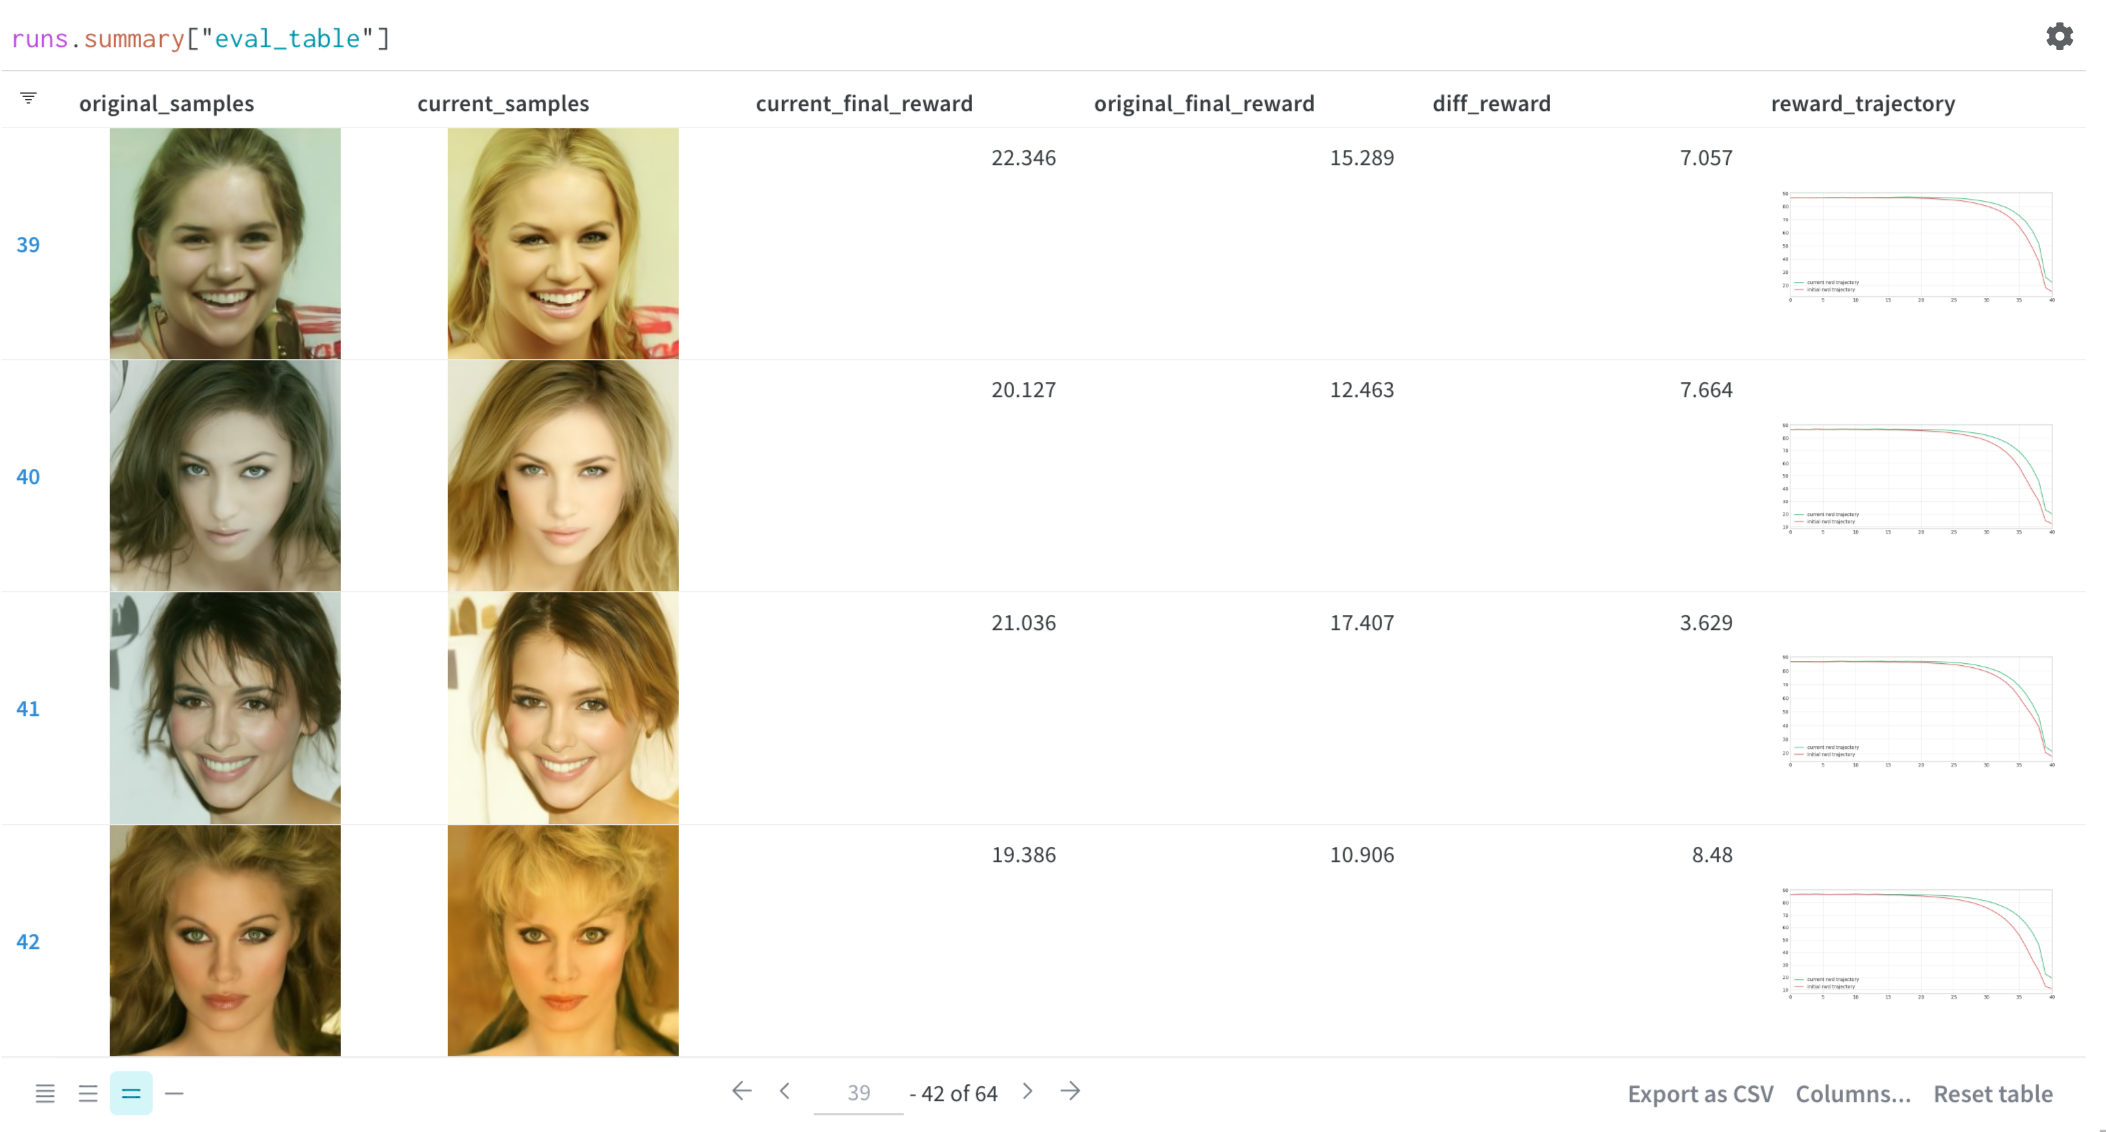
\includegraphics[scale=0.42]{img/results/devset-logging-table.png}
        \vspace{-0pt}  % reduce space between caption and figure
        \captionsetup{width=\textwidth} % set the width of the caption
        \caption{\textbf{Table for Monitoring Development Set Progress.} This table compares images generated by the pretrained model with those refined using DDPO. It displays rewards for each image, their differences, and a graph illustrating reward curves throughout the diffusion model's generation process.}
        \label{fig:devset-table}
    \end{figure}

    \noindent \textbf{Hyperparameters}. In Table~\ref{tab:Hyperparameters-summary} there is a summary of the hyperparameters used for finetuning the DDPM models on the JPEG Compressibility, Incompressibility, and Aesthetic Quality tasks using DDPO. \\

    % \noindent \textbf{Use model with \texttt{diffuser} library}. The model
    % finedtuned in this work were upload into Hugging Face model repositories as presented in Table~\ref{tab:experiment_details}, so there is easy to download and generate images, or build sample loop code. \ca{Afinar y quizás agregar bloque de código}. \\

    \begin{table}[ht]
        \centering
        \captionsetup{width=\textwidth} % set the width of the caption
        \caption{Hyperparameters for finetuning \href{https://huggingface.co/google/ddpm-celebahq-256}{\texttt{\texttt{google/ddpm-celebahq-256}}} on JPEG Compressibility, Incompressibility, and Aesthetic Quality tasks using DDPO.}
        \begin{tabular}{l l l l }
            \textbf{} & \textbf{Compressibility} & \textbf{Incompressibility} & \textbf{Aesthetic} \\
            \hline
            \textbf{Diffusion} & & & \\
            \small{Denoising steps ($T$)} & 40 & 40 & 40 \\
            \small{DDIMScheduler} & True & True & True \\
            \hline
            \textbf{Optimization} & & &  \\
            \small{Number of epochs} & 72 & 72 & 35 \\
            \small{Half-cycle cosine scheduler} & False & False & True \\
            \small{Initial learning rate} & 9e-8 & 9e-8 & 9e-8 \\
            \small{Peak learning rate} & 9e-8 & 9e-8 & 3.75e-6 \\
            \small{Warmup steps} & - & - & 25\% \\
            \small{Optimizer} & AdamW & AdamW & AdamW  \\
            \small{Weight decay} & 1e-4 & 1e-4 & 1e-4\\
            $\beta_1$ & 0.9 & 0.9 & 0.9 \\
            $\beta_2$ & 0.999 & 0.999 & 0.999 \\
            $\epsilon$ & 1e-8 & 1e-8 & 1e-8 \\
            \small{Gradient clip norm} & 1.0 & 1.0 & 1.0 \\
            \hline
            \textbf{DDPO} & & & \\
            \small{Batch size} & 10 & 10 & 10 \\
            \small{Samples per iteration} & 100 & 100 & 100 \\
            \small{Number of inner iterations} & 1 & 1 & 1 \\
            \small{Gradient updates per iteration} & 10 & 10 & 10 \\
            \small{Clip range probability ratio} & 1e-4 & 1e-4 & 1e-4 \\
            \small{Clip advantages} & 4.5 & 4.5 & 10 \\
        \end{tabular}
        \label{tab:Hyperparameters-summary}
    \end{table}

    \newpage

	
	\section{Additional Samples: Celebrity faces by DDPO}\label{appendix:additional-celebahq-samples}

    % \textbf{Additional samples.} A hundred additional comparable samples from the pretrained and DDPO finetuned models are provided.

        % 100 samples from the pretrained model
        \begin{figure}
            \centering
            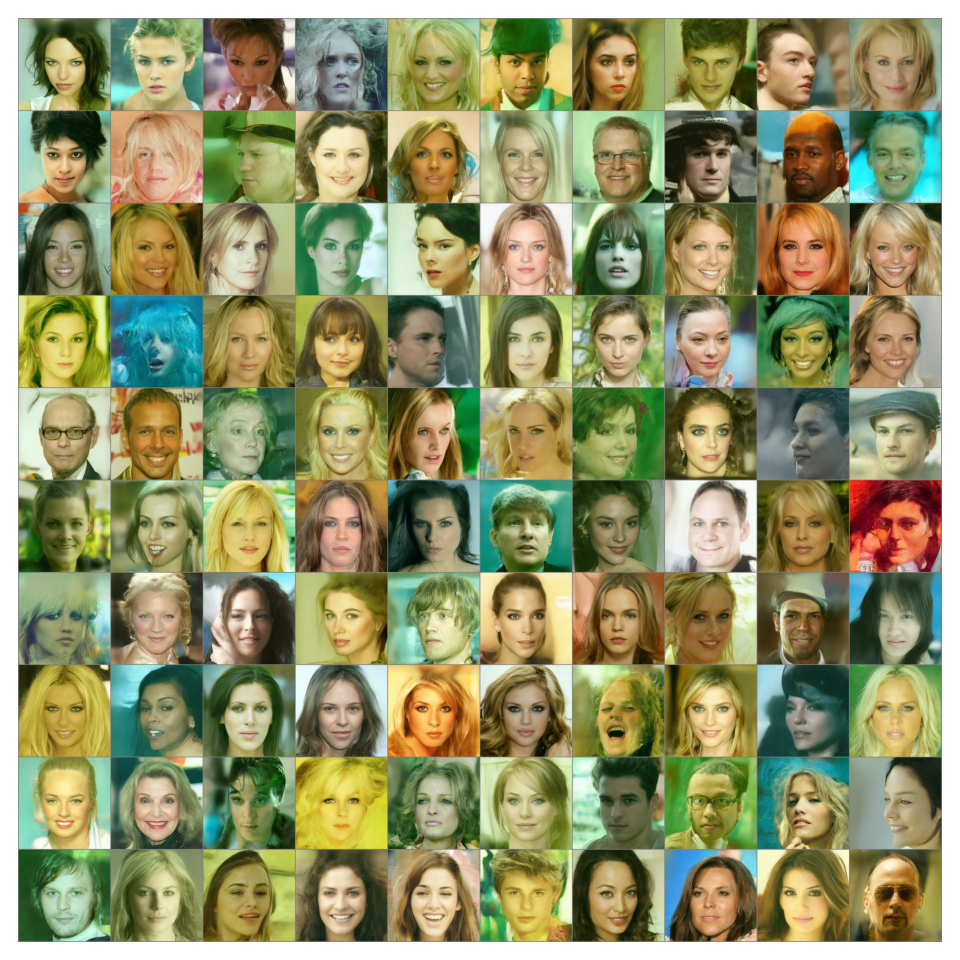
\includegraphics[scale=0.8]{img/results/ddpm-samples.png}
            \vspace{-4pt}  % reduce space between caption and figure
            \captionsetup{width=\textwidth} % set the width of the caption
            \caption{$256x\times256$ celebrity face samples generated by the pretrained model \href{https://huggingface.co/google/ddpm-celebahq-256}{\texttt{\texttt{google/ddpm-celebahq-256}}}.}
            \label{fig:ddpm-samples}
        \end{figure}

        % 100 samples from the finetuned model with ddpo and compressibility
        \begin{figure}
            \centering
            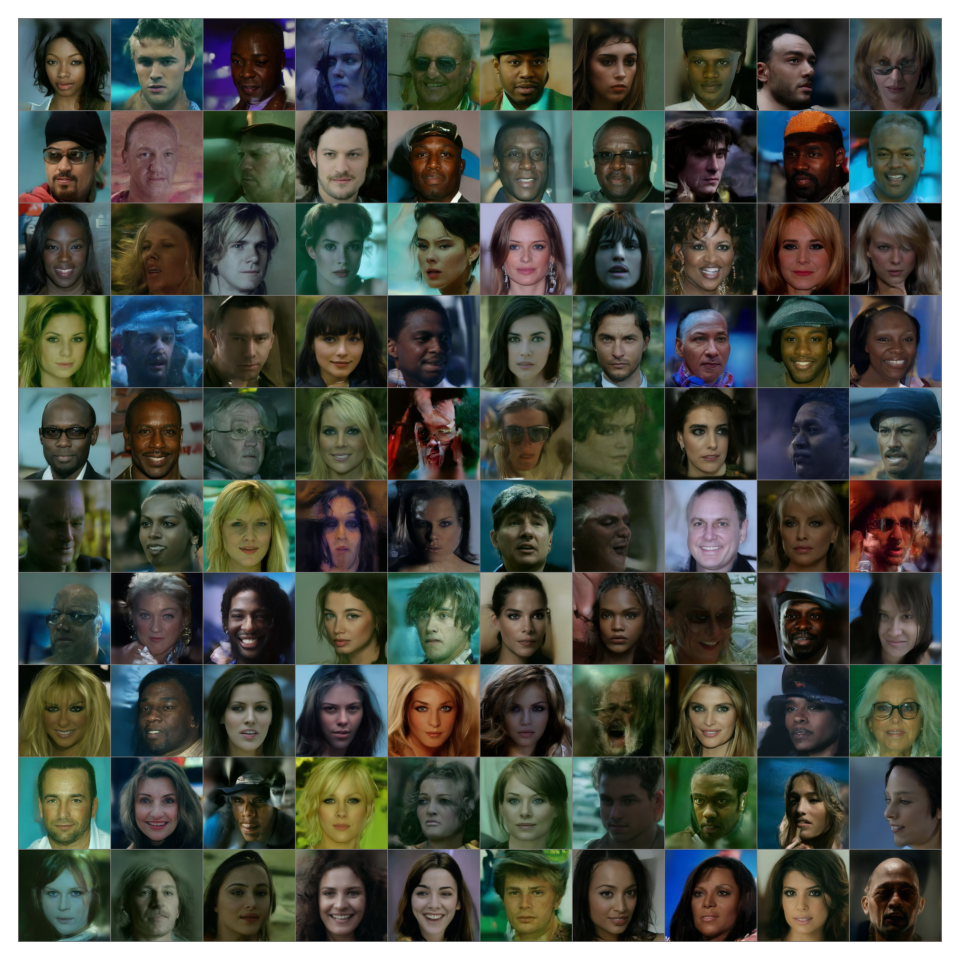
\includegraphics[scale=0.8]{img/results/ddpo-compressibility-samples.png}
            \vspace{-4pt}  % reduce space between caption and figure
            \captionsetup{width=\textwidth} % set the width of the caption
            \caption{$256\times256$ celebrity face samples generated by the DDPO finetuned model \href{https://huggingface.co/alkzar90/ddpo-compressibility-celebahq-256}{\texttt{\texttt{alkzar90/ddpo-compressibility-celebahq-256}}}, optimized for JPEG compressibility.}
            \label{fig:ddpo-compressibility-samples}
        \end{figure}

        % 100 samples from the finetuned model with ddpo and incompressibility
        \begin{figure}
            \centering
            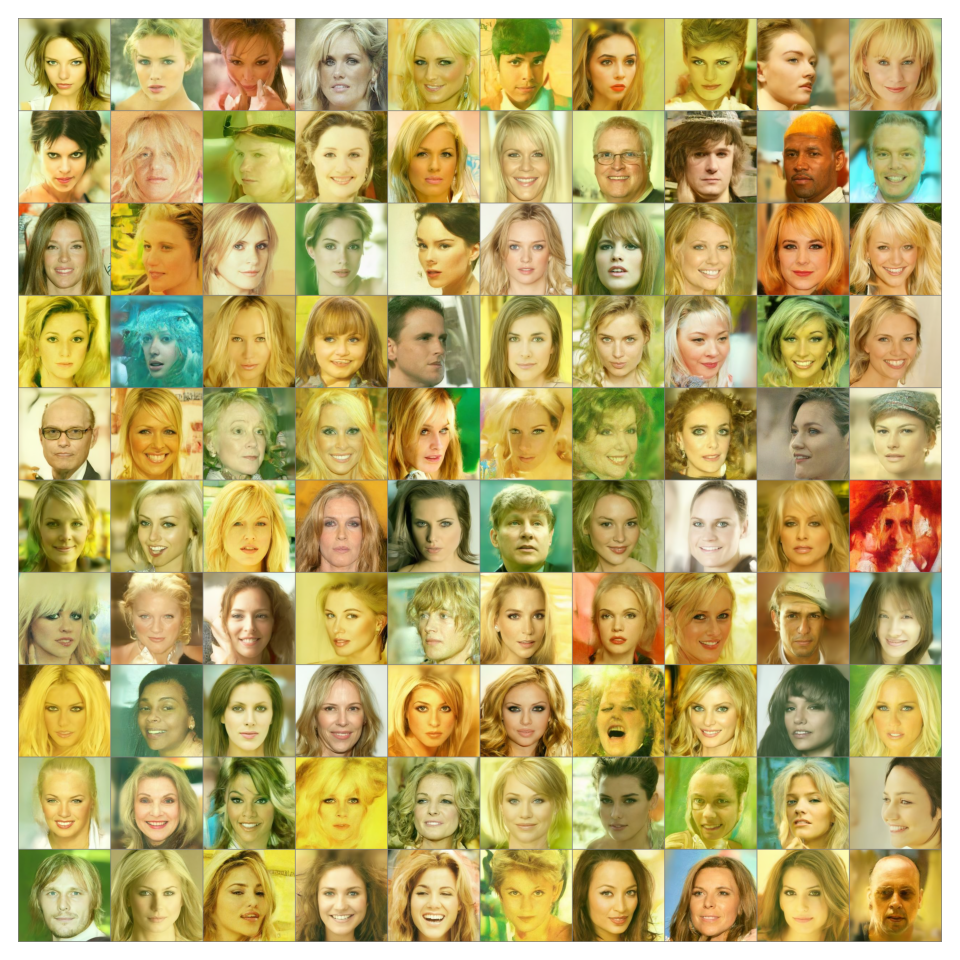
\includegraphics[scale=0.8]{img/results/ddpo-incompressibility-samples.png}
            \vspace{-4pt}  % reduce space between caption and figure
            \captionsetup{width=\textwidth} % set the width of the caption
            \caption{$256\times256$ celebrity face samples generated by the DDPO finetuned model \href{https://huggingface.co/alkzar90/ddpo-incompressibility-celebahq-256}{\texttt{\texttt{alkzar90/ddpo-incompressibility-celebahq-256}}}, optimized for JPEG incompressibility.}
            \label{fig:ddpo-incompressibility-samples}
        \end{figure}

        % 100 samples from the finetuned model with ddpo and aesthetic quality
        \begin{figure}
            \centering
            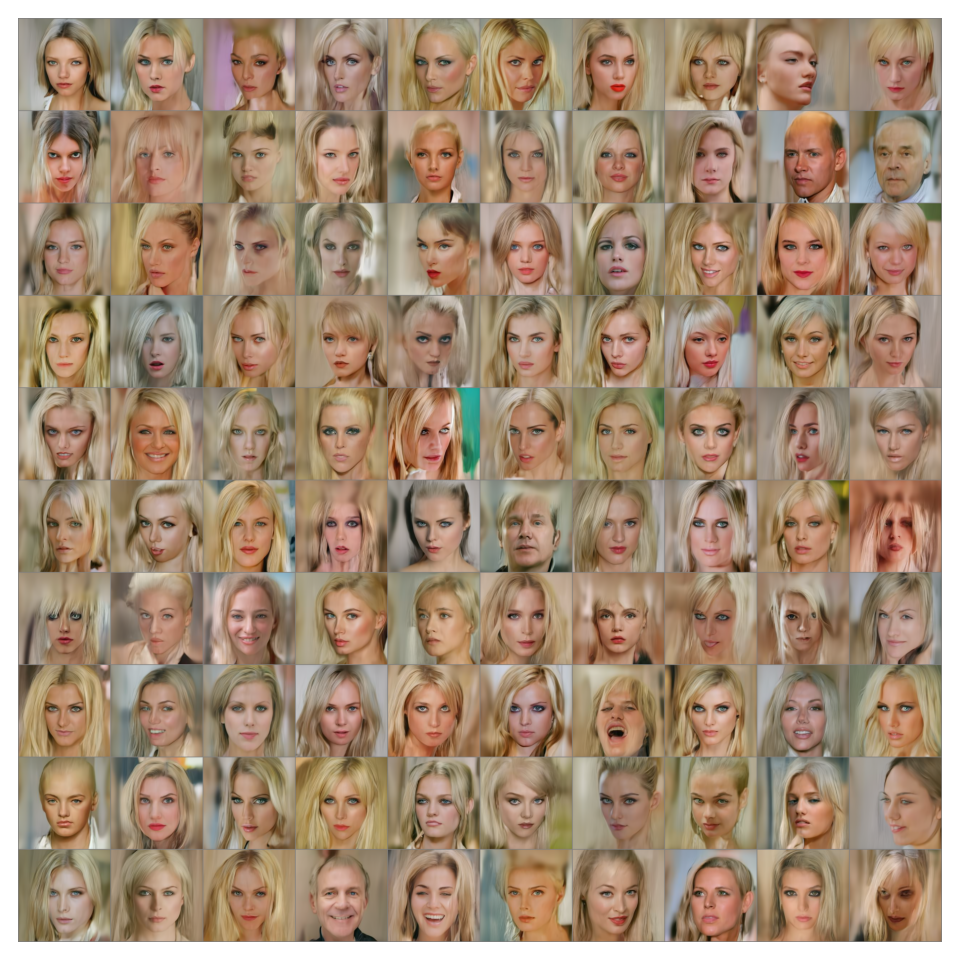
\includegraphics[scale=0.8]{img/results/ddpo-aesthetic-samples.png}
            \vspace{-4pt}  % reduce space between caption and figure
            \captionsetup{width=\textwidth} % set the width of the caption
            \caption{$256\times256$ celebrity face samples generated by the DDPO finetuned model \href{https://huggingface.co/alkzar90/ddpo-aesthetic-celebahq-256}{\texttt{\texttt{alkzar90/ddpo-aesthetic-celebahq-256}}}, optimized for aesthetic quality.}
            \label{fig:ddpo-aesthetic-samples}
        \end{figure}



    \newpage

    \section{Additional Transitions: from DDPM to DDPO}

        % transition using jpeg compressibility extra sample 1
        \begin{figure}
            \centering
            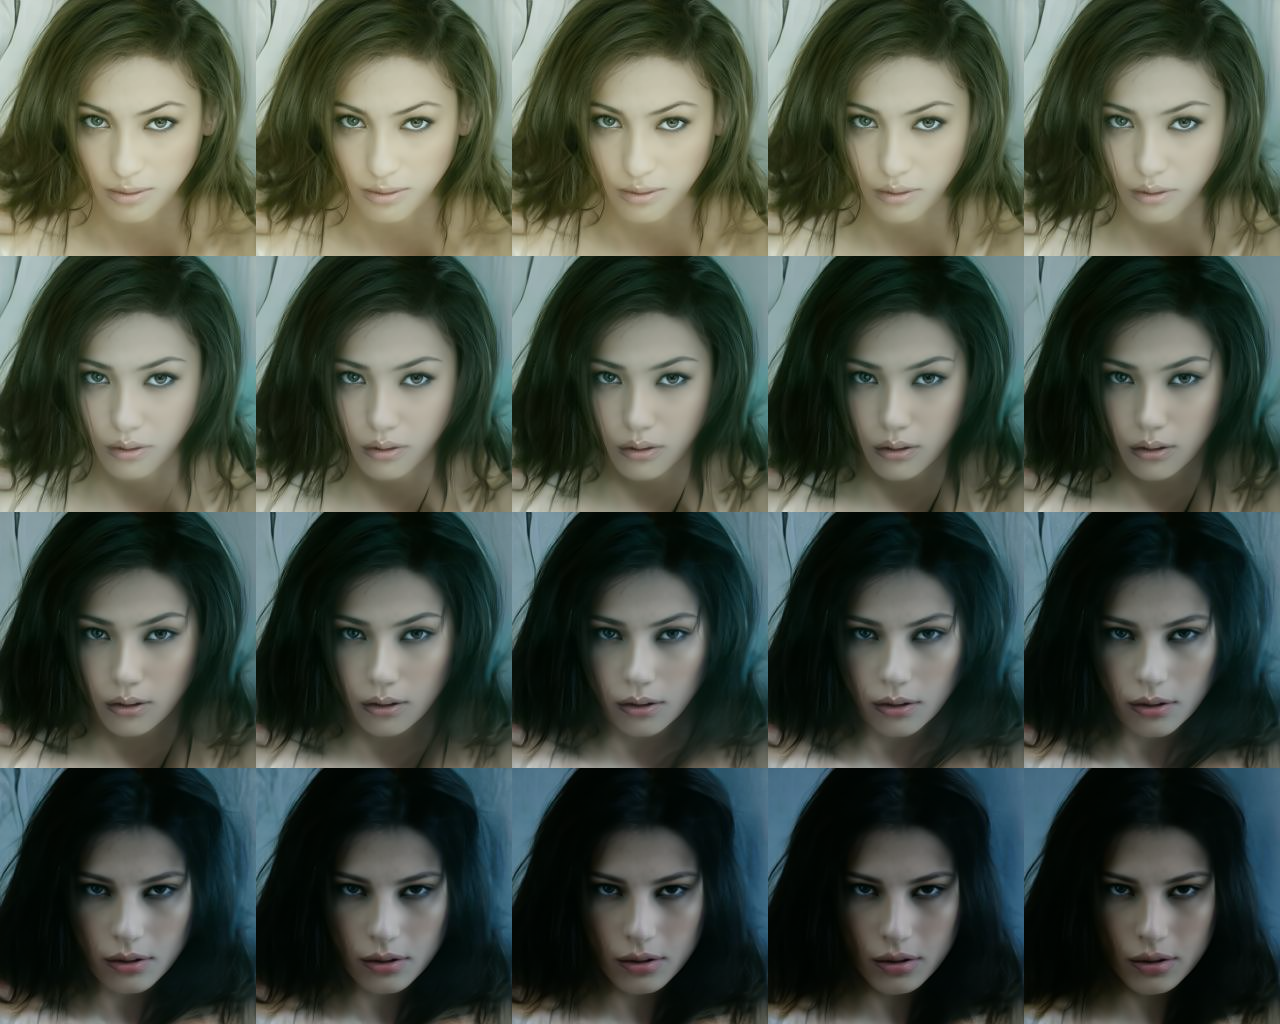
\includegraphics[scale=1.40]{img/results/compressibility_40.png}
            \vspace{-0pt}  % reduce space between caption and figure
            \captionsetup{width=\textwidth} % set the width of the caption
            \caption{\textbf{Example 1 of JPEG compressibility transformation during model updates}, starting with a pretrained DDPM model and optimized with DDPO to maximize image file size reduction after JPEG compression.}
            \label{fig:ddpm-to-ddpo-compressibility-extra1}
        \end{figure}

        % transition using jpeg compressibility extra sample 2
        \begin{figure}
            \centering
            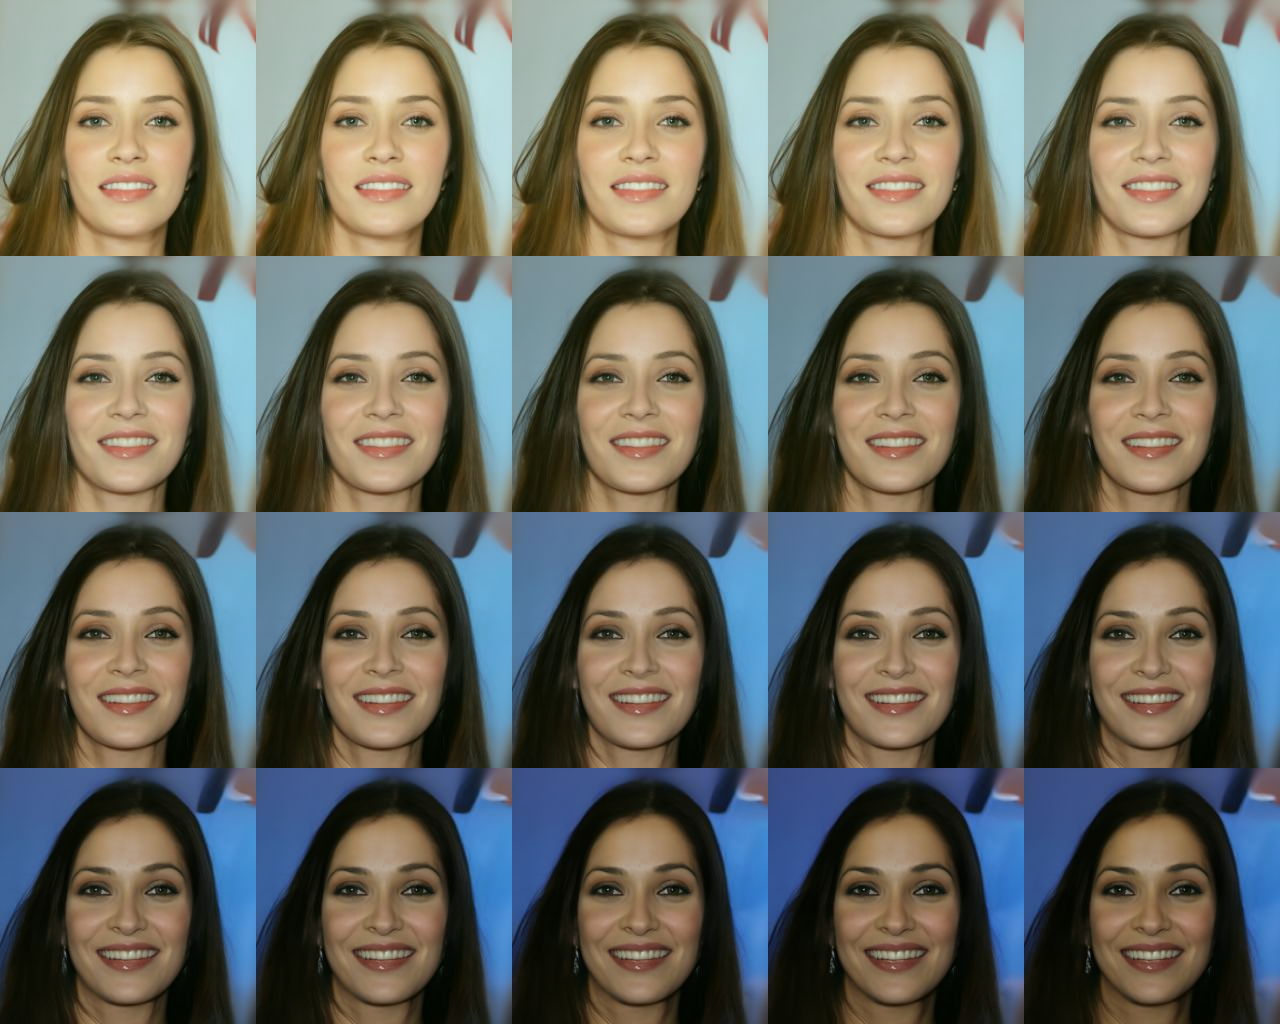
\includegraphics[scale=1.40]{img/results/compressibility_44.png}
            \vspace{-0pt}  % reduce space between caption and figure
            \captionsetup{width=\textwidth} % set the width of the caption
            \caption{\textbf{Example 2 of JPEG compressibility transformation during model updates}, starting with a pretrained DDPM model and optimized with DDPO to maximize image file size reduction after JPEG compression.}
            \label{fig:ddpm-to-ddpo-compressibility-extra2}
        \end{figure}

        % transition using jpeg incompressibility extra sample 1
        \begin{figure}
            \centering
            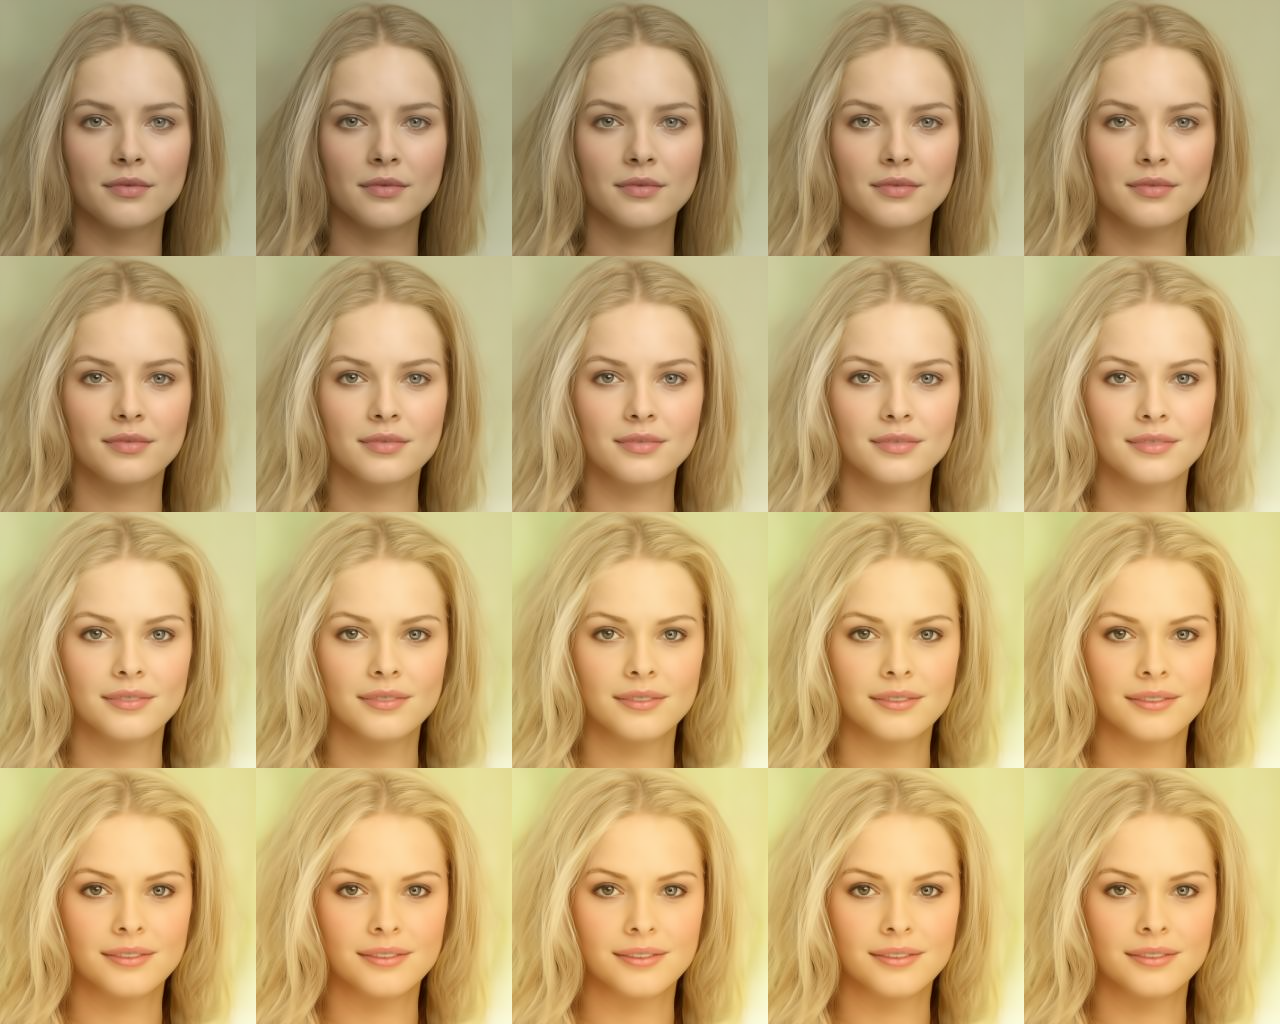
\includegraphics[scale=1.40]{img/results/incompressibility_8.png}
            \vspace{-0pt}  % reduce space between caption and figure
            \captionsetup{width=\textwidth} % set the width of the caption
            \caption{\textbf{Example 1 of JPEG incompressibility transformation during model updates}, starting with a pretrained DDPM model and optimized with DDPO to maximize image file size after JPEG compression.}
            \label{fig:ddpm-to-ddpo-incompressibility-extra1}
        \end{figure}


        % transition using jpeg incompressibility extra sample 2
        \begin{figure}
            \centering
            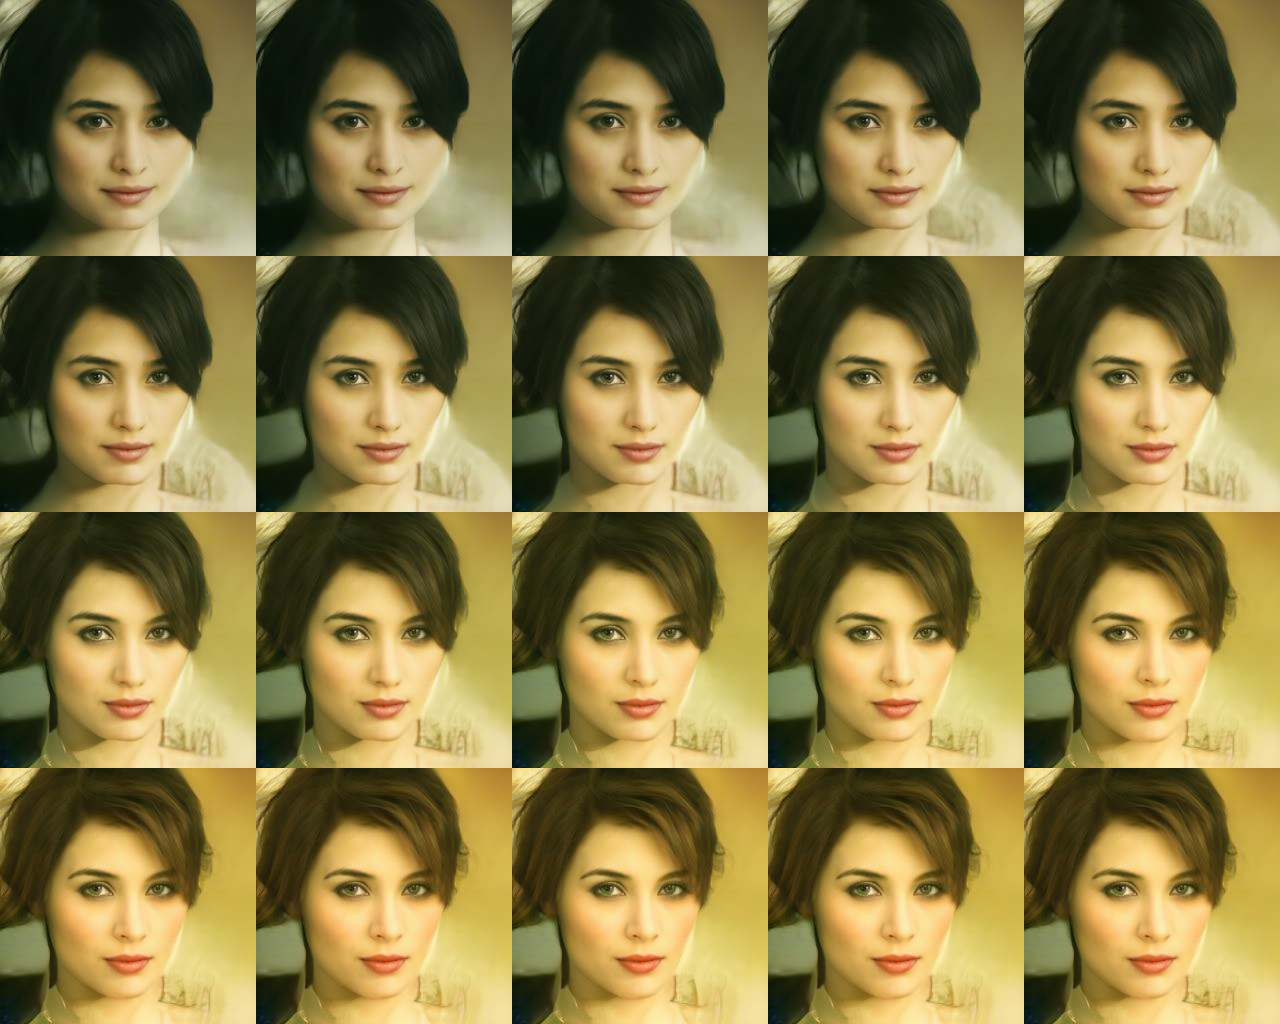
\includegraphics[scale=1.40]{img/results/incompressibility_28.png}
            \vspace{-0pt}  % reduce space between caption and figure
            \captionsetup{width=\textwidth} % set the width of the caption
            \caption{\textbf{Example 2 of JPEG incompressibility transformation during model updates}, starting with a pretrained DDPM model and optimized with DDPO to maximize image file size after JPEG compression.}
            \label{fig:ddpm-to-ddpo-incompressibility-extra2}
        \end{figure}

        % transition using aesthetic quality extra sample 1
        \begin{figure}
            \centering
            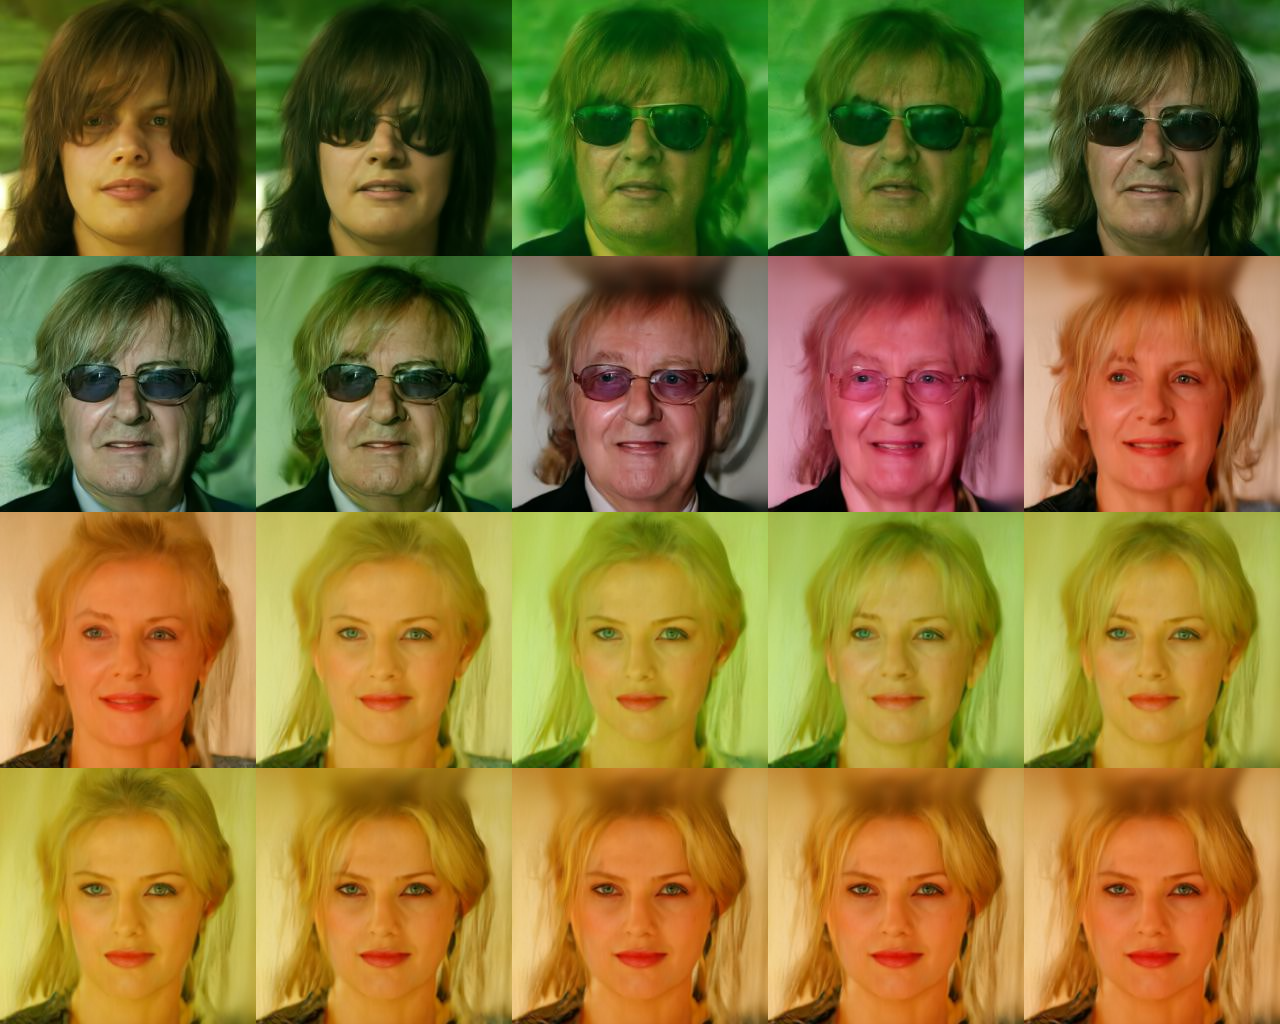
\includegraphics[scale=1.40]{img/results/laion_1.png}
            \vspace{-0pt}  % reduce space between caption and figure
            \captionsetup{width=\textwidth} % set the width of the caption
            \caption{\textbf{Example 1 of aesthetic quality transformation during model updates}, starting with a pretrained DDPM model and optimized with DDPO to maximize aesthetic quality.}
            \label{fig:ddpm-to-ddpo-aesthetic-extra1}
        \end{figure}


        % transition using aesthetic quality extra sample 2
        \begin{figure}
            \centering
            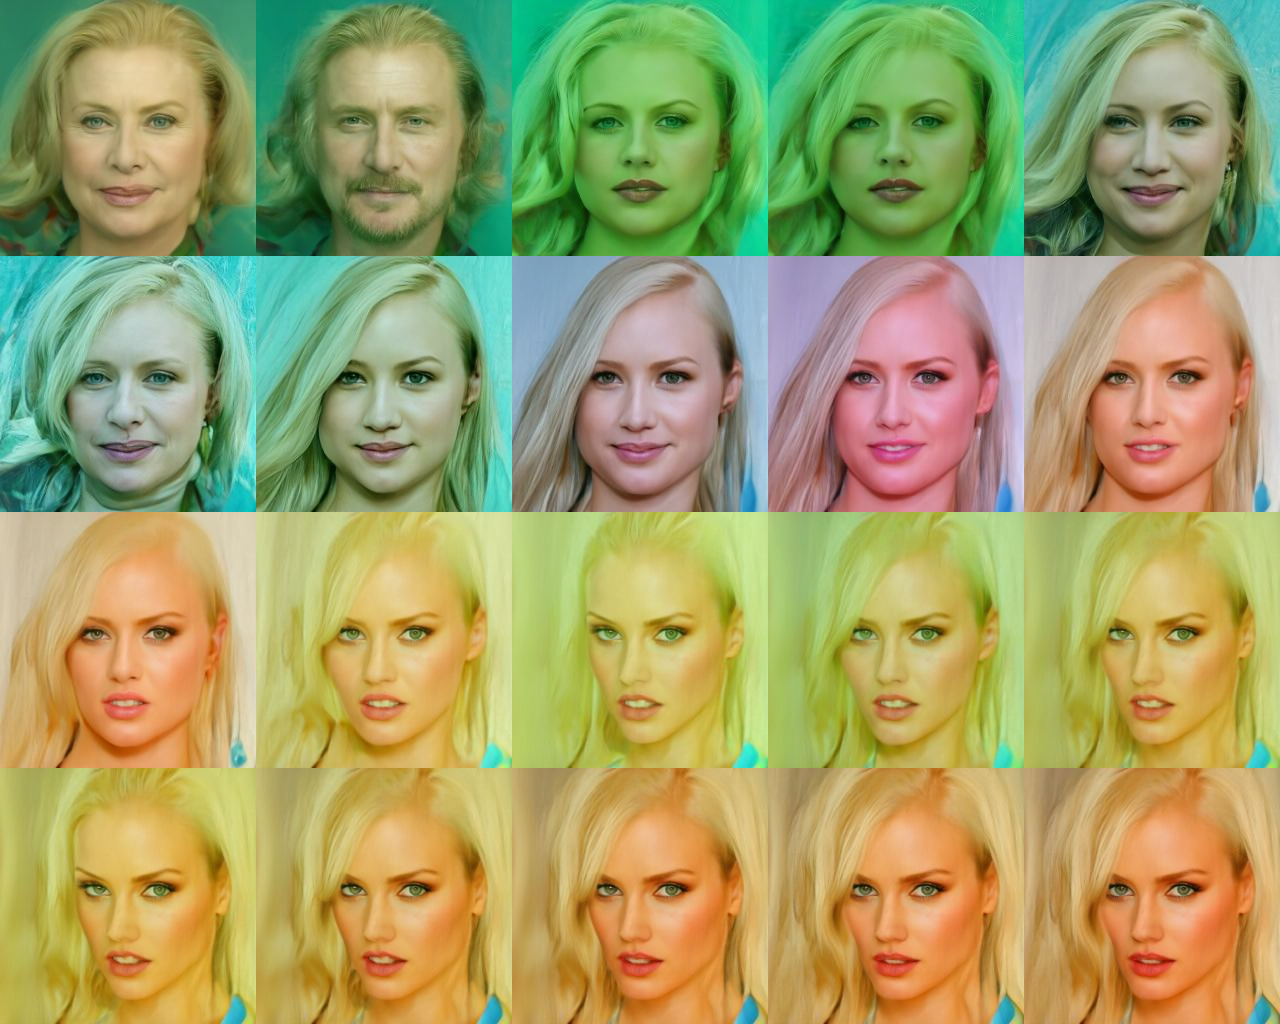
\includegraphics[scale=1.40]{img/results/laion_12.png}
            \vspace{-0pt}  % reduce space between caption and figure
            \captionsetup{width=\textwidth} % set the width of the caption
            \caption{\textbf{Example 2 of aesthetic quality transformation during model updates}, starting with a pretrained DDPM model and optimized with DDPO to maximize aesthetic quality.}
            \label{fig:ddpm-to-ddpo-aesthetic-extra2}
        \end{figure}

        % transition from DDPM to DDPO samples optimized for Task.OVER50 (ViT age classifier) extra sample 1
        \begin{figure}
            \centering
            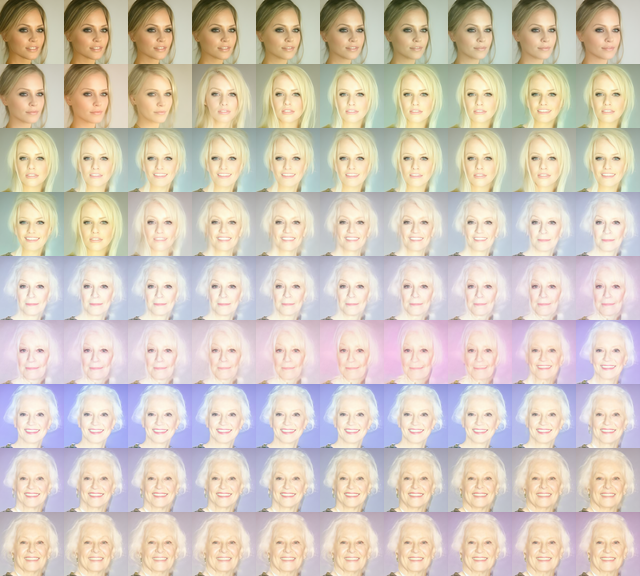
\includegraphics[scale=2.80]{img/results/over50_7.png}
            \vspace{-0pt}  % reduce space between caption and figure
            \captionsetup{width=\textwidth} % set the width of the caption
            \caption{\textbf{Example 1 of OVER50 transformation during model updates}, starting with a pretrained DDPM model and optimized with DDPO to maximize the sum of logits for classes $\geq 50$ years old using the ViT Age classifier.}
            \label{fig:ddpm-to-ddpo-over50-extra1}
        \end{figure}

        % transition from DDPM to DDPO samples optimized for Task.OVER50 (ViT age classifier) extra sample 2
        \begin{figure}
            \centering
            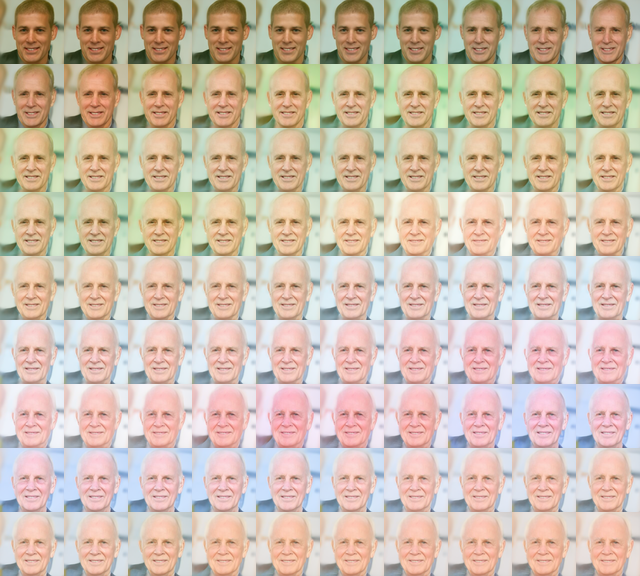
\includegraphics[scale=2.80]{img/results/over50_46.png}
            \vspace{-0pt}  % reduce space between caption and figure
            \captionsetup{width=\textwidth} % set the width of the caption
            \caption{\textbf{Example 2 of OVER50 transformation during model updates}, starting with a pretrained DDPM model and optimized with DDPO to maximize the sum of logits for classes $\geq 50$ years old using the ViT Age classifier.}
            \label{fig:ddpm-to-ddpo-over50-extra2}
        \end{figure}


    \newpage

    \section{Additional Samples: Church images by DDPO}\label{appendix:additional-church-samples}

    % \textbf{Additional samples.} A hundred additional comparable samples from the pretrained and DDPO finetuned models are provided.

        % 100 samples from the pretrained model
        \begin{figure}
            \centering
            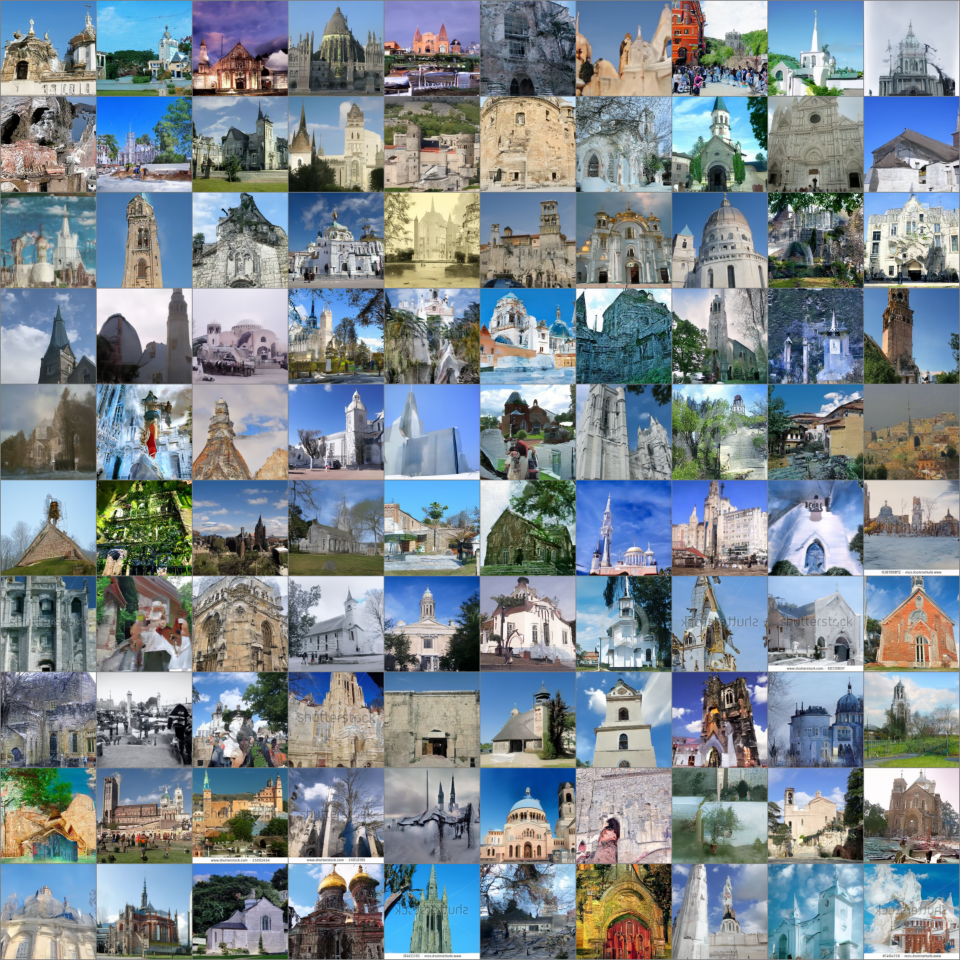
\includegraphics[scale=0.8]{img/results/ddpm-church-samples.png}
            \vspace{-4pt}  % reduce space between caption and figure
            \captionsetup{width=\textwidth} % set the width of the caption
            \caption{$256\times256$ church samples generated by the pretrained model \href{https://huggingface.co/google/ddpm-church-256}{\texttt{\texttt{google/ddpm-church-256}}}.}
            \label{fig:ddpm-church-samples}
        \end{figure}

        % 100 samples from the finetuned model with ddpo and compressibility
        \begin{figure}
            \centering
            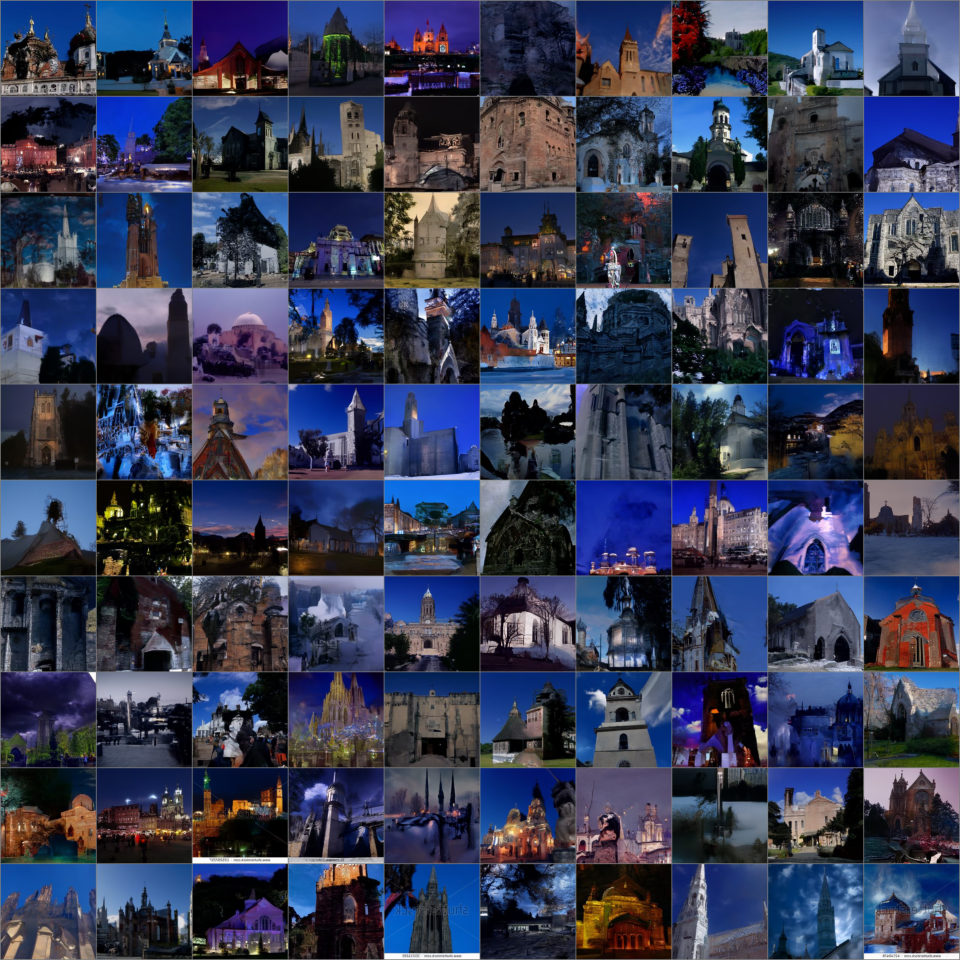
\includegraphics[scale=0.8]{img/results/ddpo-church-compressibility-samples.png}
            \vspace{-4pt}  % reduce space between caption and figure
            \captionsetup{width=\textwidth} % set the width of the caption
            \caption{$256\times256$ church samples generated by the DDPO finetuned model \href{https://huggingface.co/alkzar90/ddpo-compressibility-church-256}{\texttt{\texttt{alkzar90/ddpo-compressibility-church-256}}}, optimized by JPEG compressibility.}
            \label{fig:ddpo-church-compressibility-samples}
        \end{figure}

        % 100 samples from the finetuned model with ddpo and incompressibility
        \begin{figure}
            \centering
            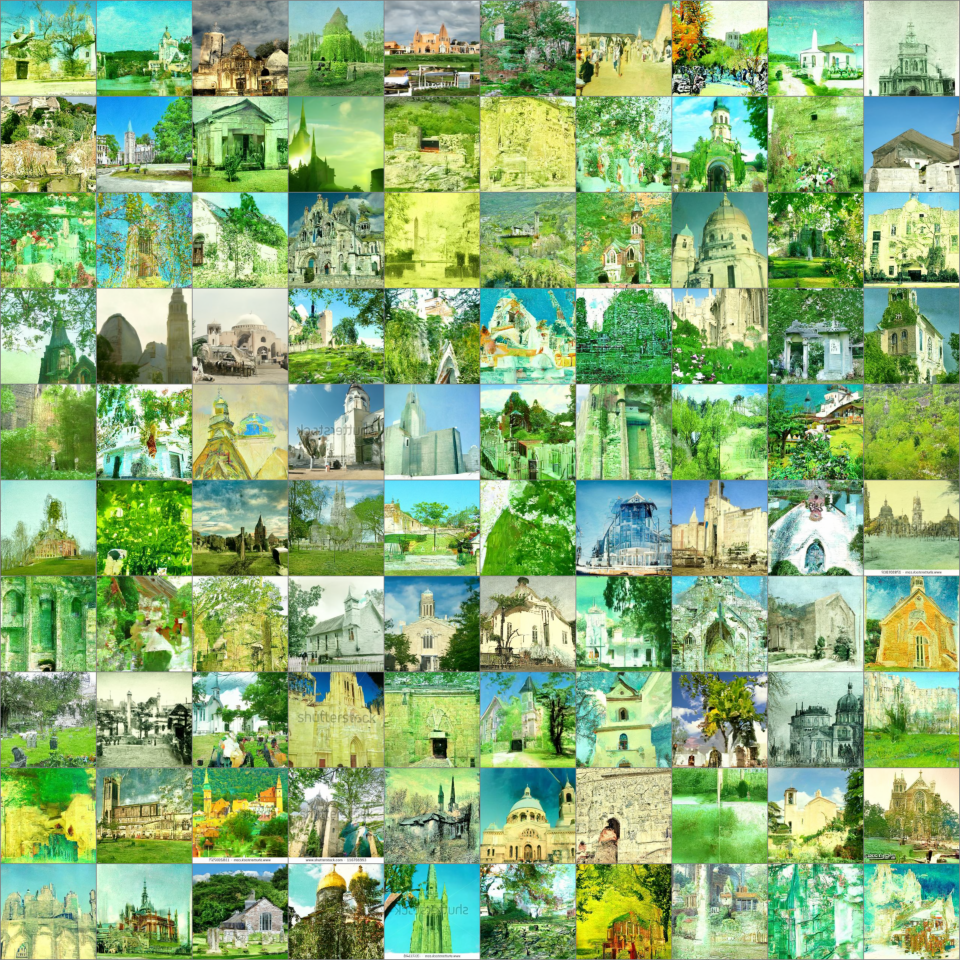
\includegraphics[scale=0.8]{img/results/ddpo-church-incompressibility-samples.png}
            \vspace{-4pt}  % reduce space between caption and figure
            \captionsetup{width=\textwidth} % set the width of the caption
            \caption{$256\times256$ church samples generated by the DDPO finetuned model \href{https://huggingface.co/alkzar90/ddpo-incompressibility-church-256}{\texttt{\texttt{alkzar90/ddpo-incompressibility-church-256}}}, optimized for JPEG incompressibility.}
            \label{fig:ddpo-church-incompressibility-samples}
        \end{figure}

        % 100 samples from the finetuned model with ddpo and aesthetic quality
        \begin{figure}
            \centering
            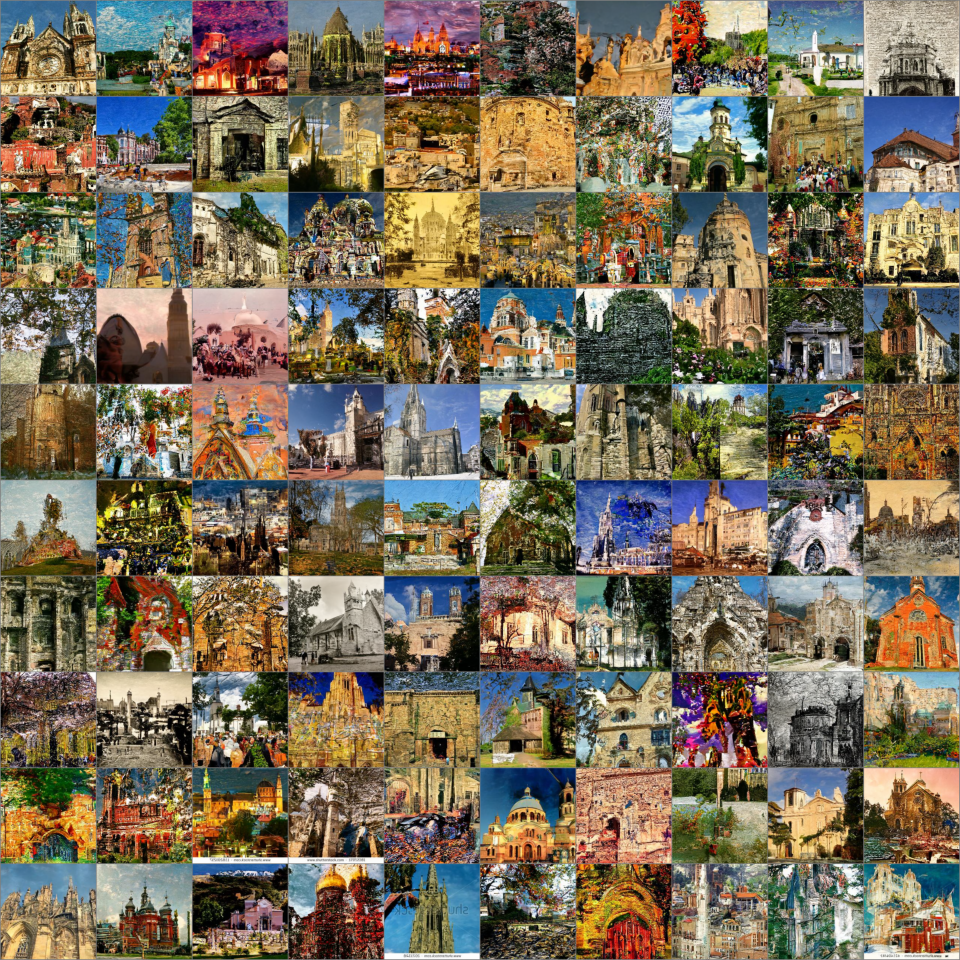
\includegraphics[scale=0.8]{img/results/ddpo-church-aesthetic-samples.png}
            \vspace{-4pt}  % reduce space between caption and figure
            \captionsetup{width=\textwidth} % set the width of the caption
            \caption{$256\times256$ church samples generated by the DDPO finetuned model \href{https://huggingface.co/alkzar90/ddpo-aesthetic-church-256}{\texttt{\texttt{alkzar90/ddpo-aesthetic-church-256}}}, optimized for aesthetic quality.}
            \label{fig:ddpo-church-aesthetic-samples}
        \end{figure}

\end{appendixs}